\chapter{Проектирование детекторов}\label{ch:detectors}

\section{Проектирование компактного орбитального детектора протонов и электронов}\label{sec:detectors/satellite}

\subsection{О солнечных космических лучах}

Более 70 лет известно, что Солнце эпизодически испускает высокоэнергичные заряженные частицы~\cite{forbush1946three}. В результате спорадических явлений солнечной активности, таких как вспышки и корональные выбросов массы (КВМ), электроны/ионы могут ускоряться до энергий в десятки МэВ/ГэВ соответственно~\cite{miroshnichenko2015solar}. Такие частицы принято называть солнечными космическими лучами (СКЛ). В некоторых довольно редких случаях потоки и энергии ионов (преимущественно протонов) СКЛ достаточны для того, чтобы породить каскад ядерных реакций в атмосфере Земли, в результате которого вторичные частицы достигают поверхности планеты и измеряются наземными детекторами. Эти события называют событиями наземных возрастаний (или GLE от “Ground Level Event”) релятивистских СКЛ. С момента первого наблюдения (в 1942 г.) зафиксировано всего 73 таких события. Намного чаще события СКЛ детектируются приборами на борту космических аппаратов (КА). Обычно энергии электронов и протонов, регистрируемых на борту КА, ограничены сверху десятками и сотнями МэВ соответственно, что во многом определяется ограниченной чувствительностью приборов (в силу ограничений на массо-габаритные характеристики), выводимых в космическое пространство. Далеко не во всех вспышечных событиях ускорение частиц происходит до таких высоких энергий. Солнечных протонных событий с энергиями выше 10 МэВ было зафиксировано намного больше (более 260, начиная с 1976 г.), чем GLE.

Несмотря на многолетнее интенсивное исследование СКЛ остается еще масса неразрешенных вопросов. До сих пор нет окончательного понимания механизмов ускорения частиц, их выхода из солнечной короны и распространения в межпланетной среде~\cite{miroshnichenko2015solar, lin2011energy}. Детальное понимание этих механизмов является фундаментальной задачей, поскольку схожие физические процессы происходят во многих астрофизических объектах. Более того, это требуется для построения надежного количественного прогноза СКЛ в различных точках гелиосферы, поскольку СКЛ могут оказывать серьезное негативное воздействие как на околоземные космические системы и межпланетные станции, так и на биологические объекты на их борту~\cite{petrukovich2008, hoff2004interplanetary, iucci2005space, hu2009modeling, zeitlin2013measurements}. Повышенные дозы радиации также получают пассажиры и члены экипажей самолетов,следующих по высокоширотным маршрутам во время солнечных событий, сопровождаемых СКЛ~\cite{beck2005tepc}.

Дальнейшее развитие космической техники и освоение космического пространства требует прогресса в изучении СКЛ. Для этого необходимо проводить измерения и мониторинг энергичных частиц одновременно в различных точках гелиосферы, на различных гелиодолготах и расстояниях от Солнца~\cite{schrijver2015understanding}. В идеале, создание разветвленной сети мониторинговых космических станций, подобно сети метеорологических станций и метеозондов на Земле. Для этого, в частности, необходимо создание надежных, легких, компактных, потребляющих малую мощность детекторов энергичных частиц, способных одновременно измерять электроны и ионы в диапазонах энергий ~1-10 МэВ и ~10-100 МэВ соответственно. Измерение электронов совместно с ионами важно, поскольку обе эти популяции солнечных энергичных частиц могут наносить урон~\cite{petrukovich2008}. В силу более высоких скоростей электронов, они обычно приходят от источника на несколько минут или десятков минут раньше ионов, что может быть использовано для краткосрочного прогнозирования прихода солнечных энергичных ионов, представляющих большую опасность~\cite{posner2007up}.


 

\subsection{Конструкция телескопа}\label{subsec:detectors/construction}

Для измерения популяций солнечных энергичных частиц обозначенных энергий,
представляющих наибольшую радиационную опасность, на КА традиционно используют
телескопы энергичных частиц. Они представляют из себя наборы детектирующих
элементов (полупроводниковых детекторов - ППД и/или сцинтилляционных детекторов, просматриваемых фотоэлектронными умножителями - ФЭУ), обычно выстроенных в ряд вдоль центральной оси, совпадающей с центральным направлением поля зрения инструмента~\cite{wuest2007calibration,galperin1972}, помещенные в  защитный кожух. 

К разрабатываемому телескопу предъявляется следующие тактико-технические требования:

\begin{itemize}
    \item Детекторный блок телескопа разрабатывается исходя из принципа минимизации массогабаритных характеристик, которые должны обеспечивать возможность установки макета на платформу стандарта “CubeSat”~\cite{cubesat}. Габариты (длина-ширина-высота) блока не должны превышать 8 см х 6 см х 6 см. Масса макета БД не должна превышать 700 г.
    \item Диапазон энергий регистрируемых частиц: электроны -- от 1 до 10 МэВ, протоны -- от 10 до 100 МэВ, типовые спектры солнечных событий приведены на графике~\ref{sat:spectrum}.
    \item Энергетическое разрешение ($\frac{\Delta E}{E}$) для обоих сортов частиц в рабочем диапазоне энергий не хуже 10\%.
    \item Схема телескопа должна обладать модификационной гибкостью. В частности, она должна позволять увеличивать верхнюю границу энергии регистрируемых частиц. Составные элементы телескопа должны быть съемными и заменяемыми.
    \item Макет должен обеспечивать требуемые измерения при одновременных радиационных загрузках потоками электронов с энергией выше 1 МэВ до $10^6$ см$^{-2}$ с$^{-1}$ и протонов с энергией выше 10 МэВ до $10^6$ см$^{-2}$ с$^{-1}$; и при отношении потоков электронов и протонов обозначенных энергий до $10^6$.
    \item Схема телескопа должна обеспечивать измерения энергичных частиц при окружающем давлении, характерном для околоземного космического пространства – от $\sim 100$ нПа (в ионосфере на высоте около 400-500 км) до $\sim 1$ нПа (в солнечном ветре на 1 А.Е.) и ниже. 
    \item Телескоп должен штатно функционировать при рабочих температурах от $-30~^{\circ}C$ до $+60~^{\circ}C$.
    
\end{itemize}

\begin{figure}[t]
    \begin{center}
        \begin{minipage}[h]{0.49\linewidth}
            \center{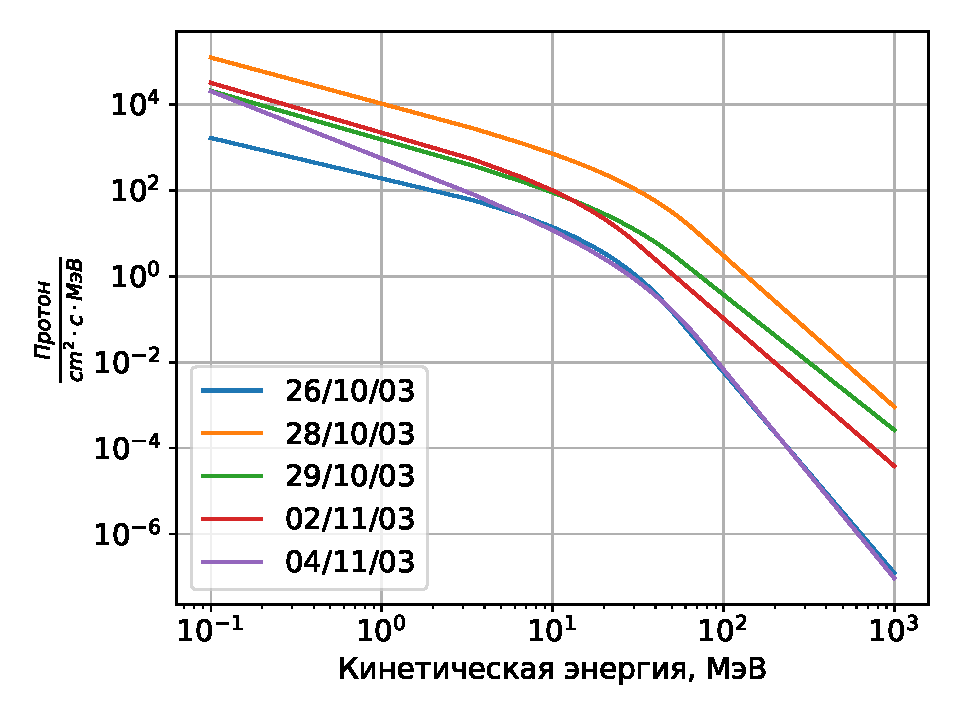
\includegraphics[width=\linewidth]{satellite/proton_spectrum.pdf} \\ а)}
        \end{minipage}
        \hfill
        \begin{minipage}[h]{0.49\linewidth}
            \center{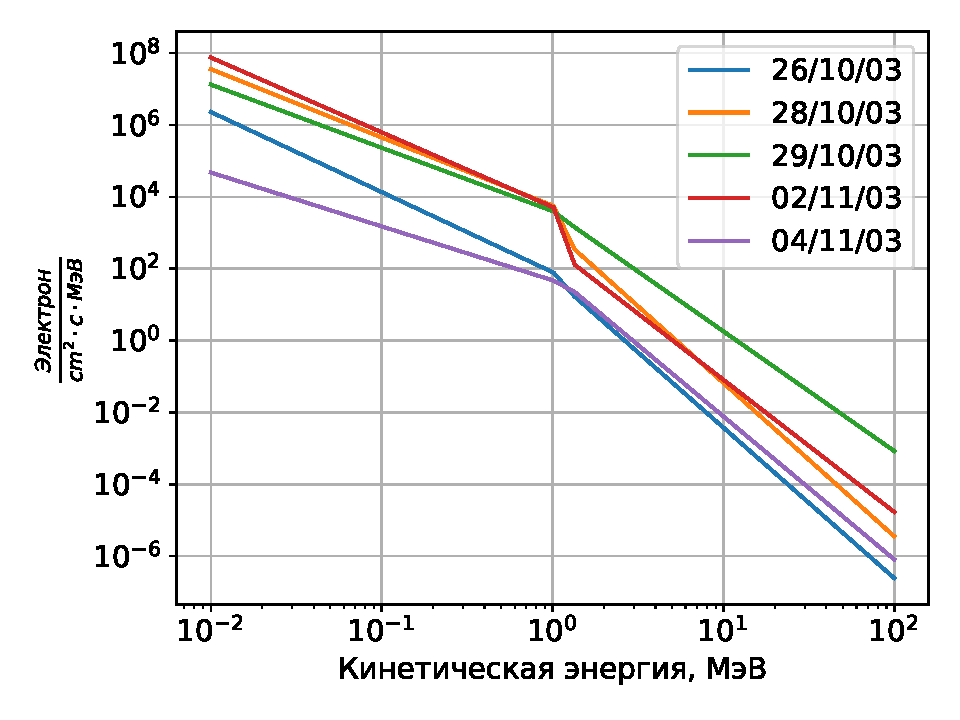
\includegraphics[width=\linewidth]{satellite/electron_spectrum.pdf}   \\ б)}
        \end{minipage}
        \caption{ Спектры в мощных солнечных событиях октября-ноября 2003 г~\cite{mewaldt2005proton}: а) протонов б) электронов.}
    \end{center}
    \label{sat:spectrum}
\end{figure}

Для выбора типа детектирующего элемента разберем насколько ППД и сцинтилляционные детекторы удовлетворяют заявленными требованиям. К преимуществам ППД можно отнести их компактность и высокую разрешающую способность~\cite{lutz2007semiconductor}. Однако недостатком единичного ППД является отсутствие пространственной чувствительности и возможности различения разных типов частиц. При современном уровне технологий более целесообразной является разработка телескопа на основе сегментированного сцинтилляционного детектора. Среди преимуществ сцинтилляционного детектора можно отметить следующие: 
\begin{itemize}
    \item Малое (порядка нескольких десятков  наносекунд для органических и сотен пикосекунд для неорганических сцинтилляторов~\cite{shendrik2013}) время высвечивания, позволяющее работать в одночастичном режиме в широком диапазоне скоростей счёта (ППД имеют проблемы при скоростях счета больше $10^4$ частиц в секунду).
    \item Более высокая радиационная стойкость и долговечность по сравнению с полупроводниковыми детекторами, возможность создавать более толстые слои материала, отсутствие подложки~\cite{shendrik2013, lutz2007semiconductor}. 
    \item Меньшее по сравнению с ППД энергетическое разрешение, тем не менее достаточное для решения поставленных перед телескопом задач~\cite{shendrik2013, lutz2007semiconductor}. 
\end{itemize} 
Одна из проблем сцинтилляционных детекторов - необходимость для регистрации сцинтилляционного света, или габаритных и хрупких  фотоэлектронных умножителей, или лавинных фотодиодов, компактных, но имеющих худшее энергетическое разрешение, решена в настоящее время благодаря созданию кремниевых фотоумножителей (SiPM), представляющих из себя матрицы из лавинных фотодиодов~\cite{akimov2006}. Также в отличии от ППД в которых  электроника для съема сигнала расположена в плоскости перпендикулярной оси наблюдения (и соответственно при создании сегментированного полупроводникового детектора будет подвержена радиационным повреждениям), съем сигнала с сцинтилляционных шайб возможен с торца шайбы или посредством оптоволоконного кабеля (что позволяет разделить рабочее тело детектора и электронику, укрыв её в корпусе КА). За счет сегментации детектора и раздельного съема света с разных слоев, можно частично идентифицировать геометрию трека частицы и фильтровать события в нужном апертурном окне без использования громоздких коллиматоров. Однако небольшое апертурное устройство для выделения необходимого поля зрения помогает улучшить характеристики детектора, так же возможна установка фильтра низкоэнергетичных частиц (например, бериллиевого покрытия).

\begin{figure}[ht]
    \centerfloat{
        \hfill
        \subbottom[Ионизационные потери для протонов (100 МэВ) и электронов (10 МэВ)\label{sat:bragg}]{%
            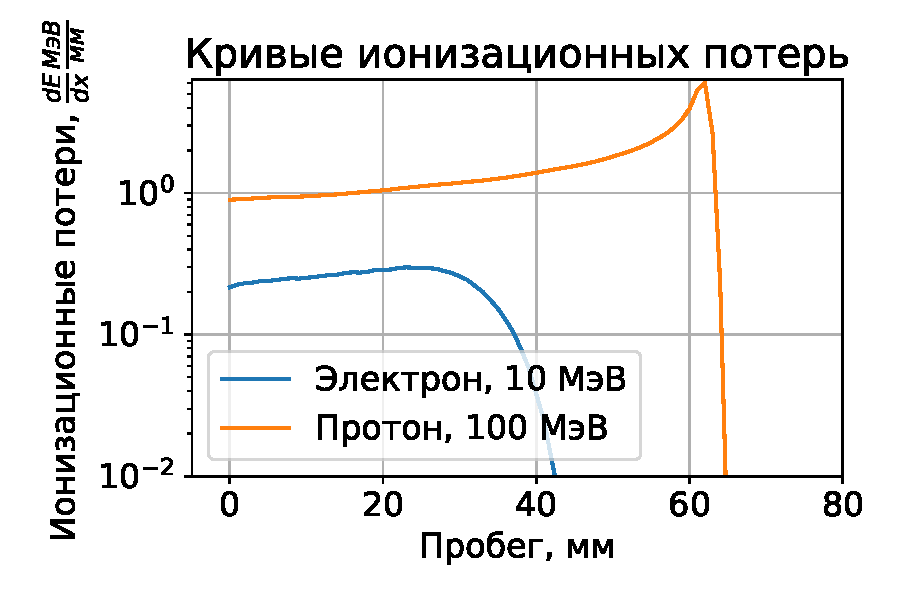
\includegraphics[width=0.4\linewidth]{satellite/01_bregg.pdf}}
        \hfill
        \subbottom[Пробег протонов и электронов\label{sat:range}]{%
            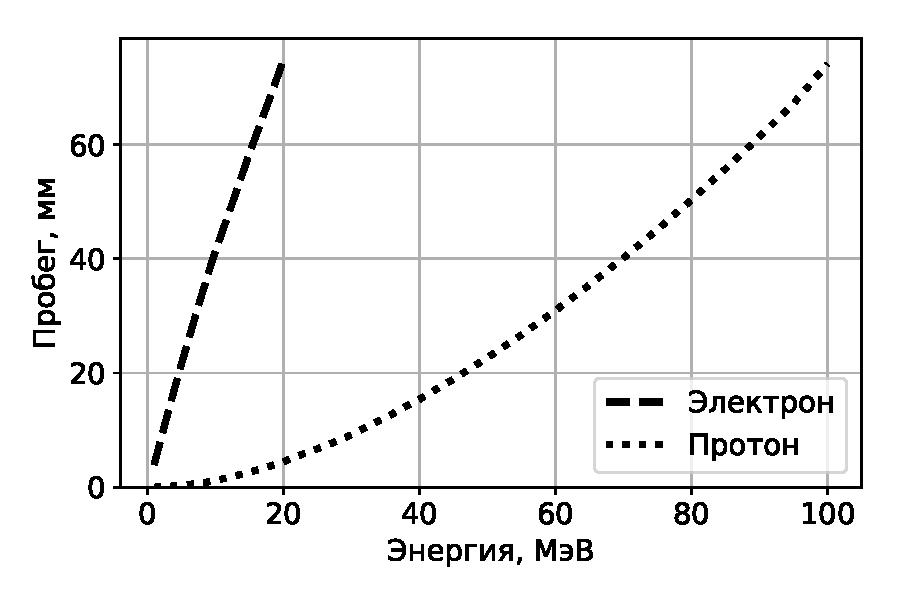
\includegraphics[width=0.4\linewidth]{satellite/lebedev/02_range.pdf}}
        \hfill
    }
    \caption{Прохождение протонов и электронов через антрацен}\label{sat:antrachen}
\end{figure}

Создание многослойного сцинтилляционного детектора позволяет проводить анализ не только по полной выделенной энергии, но и по форме кривой зависимости   ионизационных потерь  от пробега частицы, а также отсекать фоновые события, анализируя расположения сработавших слоев. На рисунке~\ref{sat:antrachen}а показаны зависимости для потерь на единицу длины в зависимости от глубины проникновения для протонов с энергией 100 МэВ и для электронов с энергией 10 МэВ. Следует отметить два факта - кривые ионизационных потерь протонов имеют характерную особенность - пик Брэгга и разницу в ионизационных потерях протонов и электронов, что позволяет, измерив зависимость энерговыделения от пробега с высокой точностью определить тип и энергию частицы~\cite{Gruppen}. Полная длина пробега электронов и протонов в антрацене (он выбран как типовой пластиковый сцинтиллятор, рассуждения приведенные ниже аналогичным образом легко повторить для других веществ, например полистирола) приведена на рисунке. Пробег протонов с энергией 100 МэВ около 65 мм. Причем если мы возьмем данный пробег в качестве полной длины детектора мы сможем эффективно измерять энергию протонов вплоть до 150 МэВ,  благодаря информации о форме кривой Брэгга, или же напротив мы можем сократить длину детектора, ухудшив диапазон измеряемых энергий, но при этом сократив массу. Также исходя из этого графика можно рекомендовать делать первые наиболее тонкие слои не более двух миллиметров для обеспечения эффективной регистрации электронов. Толщины наиболее толстых слоев должны быть достаточными для поглощения пика Брэгга и быть в диапазоне 5 -10 мм. Радиус детектора целесообразно подбирать из диапазона 10 - 50 мм. Исходя из данных геометрических оценок масса без учета электроники может лежать в пределах 200-800 грамм.

При этом предполагаются три режима работы детектора, при низкой скорости набора событий производится анализ каждого одиночного события, а при превышении некоторого порога (обусловленного скоростью работы электроники и временем высвечивания сцинтиллятора) идет накопление суммарных потерь за некоторый промежуток времени, а затем восстанавливается энергетический спектр частиц попавших в детектор за это время. Третий режим является смешанным: в шайбах расположенных вблизи входного окна проводится измерение суммарных ионизационных потерь, а в дальних шайбах производится идентификация отдельных событий (это возможно при условии, что число частиц составляющих более высокоэнергетичных часть спектра будет меньше чем пороговая скорость счета). В качестве основы для анализа используется рассчитанные значения ионизационных потерь и набор триггеров для отсечения событий. Надо отметить, что детектор позволяет также измерять более тяжелые частицы (ионы) и отличать их от протонов (энергетический диапазон при этом сдвигается в область высоких энергий), а также с пониженной эффективностью частицы сверхвысоких энергий и гамма-кванты.

Среди достоинств выбранной схемы можно отметить широкую адаптивность сборки. В зависимости от конкретной задачи и ограничений на габариты и вес прибора, можно варьироваться следующие параметры:
\begin{itemize}
    \item Полная длина телескопа --- увеличение полной длины детектора приводит к увеличению измеряемого диапазона энергий, но и увеличивает массу детектора. Надо отметить, что детектор позволяет измерять энергию частиц, которые проходят его насквозь (при помощи определения потерь на единицу длины), но точность этих измерений существенно ниже.
    \item Радиус детектора --- увеличение радиуса позволяет более точно определять энергию электронов (из-за того что электроны сильно рассеиваются, часть электронов может покидать узкий телескоп через боковые стенки, исказив энерговыделение), а также увеличивает угловую апертуру, но существенно увеличивает вес. 
    \item Количество отдельных слоев и их толщины --- с одной стороны увеличение количества слоев улучшает пространственное разрешение, с другой в более тонких слоях заметнее флюктуации ионизационных потерь. Тонкие слои необходимы вблизи входного окна поскольку там требуется большая точность определения формы кривой потерь для лучше разрешения низкоэнергетичных частиц, но в тоже время сложнее в изготовлении и менее устойчивы к износу и механическим вибрациям. Так же увеличение количества слоев увеличивает вес электроники.
    \item Тип сцинтиллятора --- очень многогранный параметр, влияющий не только на эффективность регистрации частиц, но и на массо-габаритные характеристики: более плотные сцинтилляторы позволяют создавать более компактный детектор (но и усложняют изготовления из-за уменьшения толщины отдельного слоя). Также следует учесть ограничения по температурам и радиационной нагрузки, которые зависят от конструкции спутника и решаемых им задач.
\end{itemize}
Подобная вариативность хорошо показывает необходимость моделирования конструкции детектора перед его воплощением в железе, перебирая различные наборы параметров можно найти наиболее оптимальное для заданной задачи соотношение. Далее в работе мы покажем как на основе моделирования оценить параметры детектора для одночастичного и интегрального режимов работы и приведено описание методик обработки сигнала для этих режимов. В дальнейших разделах для расчета энерговыделения в сцинтилляционных шайбах проведено GEANT4 Монте-Карло моделирование при этом  использовался конструктор \textit{G4EmStandartPhysics}.

\subsection{Одночастичный режим}
В одночастичном режиме анализ проводится следующим образом. Для анализа отбираются события прошедшие через входное окно (иначе говоря инициирующие срабатывания сцинтилляторов начиная с первого слоя). После чего исходя из полной измеренной энергии и количества сработавших слоев определяется диапазоны возможных параметров частицы, а также отсекаются события пришедшие под большими углами. В данных диапазонах параметров определяется набор параметров максимизирующей значение функции правдоподобия --- произведения вероятностей наблюдать измеренное энерговыделение при данном наборе параметров. Процедура восстановления энергии в настоящее время дорабатывается, но предварительный алгоритм позволяет определить энергию протонов с точностью 1 МэВ для исходной энергии 50 МэВ, то есть дает точность порядка 2\%. Предполагается, что в дальнейшем точность восстановления будет улучшена в 1.5 - 2 раза за счет фильтрации событий под большими углами. Реальная чувствительность будет несколько меньше за счет неидеальности светосбора и уменьшения количества шайб, но при любых конфигурациях детектора, разрешающая способность детектора будет не хуже 10\%.
\subsection{Интегральный режим}
Для анализа спектра в интегральном режиме будет использоваться методика регуляризации обратных задач, разработанная В. Ф. Турчиным, которая позволяет без потери точности строить решение обратной интегральной задчи. Другими словами, она позволяет из интегрального спектра, содержащего протоны и электроны разной энергии выделять дифференциальные спектры для различных типов частиц. В качестве референсных кривых поглощения для восстановления используются данные моделирования. В дальнейшем планируется для этого использовать данные калибровочных измерений на протонном ускорителе Московской Мезонной Фабрики в Троицке.
В настоящее время проводится доработка математического аппарата и программной базы для анализа в интегральном режиме. Предварительные результаты восстановления спектра дают точность до 5\% в зависимости от диапазона измерений. Важно отметить, что интегральная методика применима при очень высоких загрузках детектора (свыше 1 МГц).
\subsection{Обсуждение результатов}
Разработана концепция секционного сцинтилляционного телескопа для регистрации электронов и протонов солнечного происхождения. Произведены работы по моделированию детектора и сделаны оценки его чувствительности для различных частиц и в различных диапазонах энергий. Предварительные результаты показывают, что при весе до 1 кг, детектор сможет позволить измерение энергетического спектра протонов от 5 до 100 МэВ и электронов от 1 до 10 МэВ с точностью порядка 1-5\%.
Существенным преимуществом детектора является возможность работы в так называемом интегральном режиме, когда не регистрируются индивидуальные частицы, а идет анализ полного пространственного спектра потерь энергии. Интегральный режим позволяет работать при сверхвысоких скоростях счета, обеспечивая при этом достаточно хорошую (около 5\%) точность восстановления исходного спектра и состава излучения.



\section{Проектирование сканеров основанных на использовании рентгеновского и гамма излучения
}\label{sec:detectors/scanners}

\todo{Пересказать этот раздел другими словами что бы не считалось плагиатом из статьи}

Для обеспечения национальной безопасности важен контроль перемещения опасных или стратегически важных грузов, таких как взрывчатые вещества, радиоактивные материалы, редкие и драгоценные металлы. Проводить такой контроль можно, сканируя содержимое транспортных контейнеров гамма-излучением.

В данной работе рассмотрена существующая методика дуальных энергий и предложен альтернативный способ, основанный на измерении энергетического распределения гамма-квантов. Для оценки было проведено моделирование с помощью транспортного кода GEANT4.  Также выполнен эксперимент по измерению энергетического разрешения детектора на основе сцинтиллирующего кристалла BGO и кремневого фотоумножителя.

Использование высокоэнергетического гамма-излучения в прикладной томографии на данный момент широко распространено.  В этой статье мы рассмотрим возможности улучшения существующего метода как путем модернизации оборудования, так и путем разработки математических алгоритмов, которые более полно используют информацию, содержащуюся в измеренных значениях. В начале мы рассмотрим существующий метод дуальных энергий и определим возможные направления для создания более точной методики. Далее в работе приведено описание нескольких симуляций и численных экспериментов с обсуждением результатов. Также в работе приведены результаты измерений характеристик сцинтилляционного кристалла BGO, который может послужить основой для модернизированного оборудования.
 
\subsection{Метод дуальных энергий}
\begin{figure}[t]
    \begin{center}
        \begin{minipage}[h]{0.49\linewidth}
            \center{ \includegraphics[width=0.99\linewidth]{scanner/Attenuation.pdf}  \\ а)}
        \end{minipage}
        \hfill
        \begin{minipage}[h]{0.49\linewidth}
            \center{ \includegraphics[width=0.99\linewidth]{scanner/Bremsstrahlung.pdf}  \\ б)}
        \end{minipage}
        \caption{а) Массовый коэффициент ослабления для различных материалов. б) Спектр тормозного излучения от электрона с энергией 10 МэВ.}
    \end{center}
    \label{pic:att}
\end{figure}

Рассмотрим, как уменьшается поток гамма-лучей. Коэффициент пропускания описывается следующим уравнением:
\begin{equation}
\label{eq:trans}
T(E_0, t, Z) = \frac{\int \limits_0^{E_0} S(E_0, E) \exp(-\mu(E,Z)\times t)~dE)}{\int \limits_0^{E_0} S(E_0, E)~dE},
\end{equation}
где $T$ --- прозрачность материала для гамма-излучения, $S(E_0, E)$ --- функция отклика детектора, $\mu(E,Z)$ --- массовый коэффициент ослабления, $t$ ---  оптическая толщина материала, $E_0$ --- предельная энергия тормозного излучения, $E$ --- энергия гамма-излучения, $Z$ --- заряд ядра исследуемого материала.

Предположим, что в качестве источника гамма-лучей используется тормозное излучение со спектром как на рисунке~\ref{pic:att}б и максимальной энергией $E_0$, зависящей от энергии электронного пучка. Коэффициент прозрачности  $T(E_0, t, Z)$ также зависит от среднего массового коэффициента ослабления материала. Рисунок~\ref{pic:att}а показывает зависимость коэффициента ослабления от энергии для различных материалов. Мы можем выделить три области: начальную, в которой доминирует фотоэлектрический эффект и могут быть разделены только материалы с большим зарядом ядра; среднюю, в которой доминирует комптоновское рассеяние и материалы не различимы,и наконец область, где основное влияние оказывает процесс рождения электрон-позитронных пар и материалы достаточно хорошо различимы~\cite{geheitler1984quantum, spirin, Geant2016}. Последняя область может быть использована для метода дуальных энергий~\cite{spirin}.

Уравнение~\ref{eq:trans} не позволяет определить материал, если неизвестна оптическая толщина материала. Для решения этой проблемы в методе дуальной энергии предлагается использовать два электронных пучка с различной энергией. Используя прозрачность для двух предельных энергий гамма-лучей $E^{(1)}_0$ и $E^{(2)}_0$, а затем минимизируя функционал
\begin{equation}
F(z) = \frac{|t(E^{(1)}_0,z) - t(E^{(2)}_0,z)|}{t(E^{(1)}_0,z)} \to min,
\end{equation}
становиться возможным исключить неизвестную нам оптическую толщину и вычислить эффективное зарядовое число для исследуемого материала. Данный метод позволяет отнести сканируемый материал к одной из четырёх групп, разделённых по эффективному зарядовому числу: $Z_{eff} \sim 5$, $Z_{eff} \sim 13$, $Z_{eff} \sim 26$, $Z_{eff} \sim 82$.\\
Однако, метод дуальной энергии имеет некоторые недостатки, среди которых мы выделим два:
\begin{itemize}
    \item Необходимость в двух пучках различной энергии ведет к усложнению конструкции сканера.
    \item Данный метод будет иметь малую эффективность в случае материала, состоящего из сильно различающихся по заряду элементов.
\end{itemize}
Поэтому мы предлагаем альтернативный подход:
\begin{itemize}
    \item Использовать только один электронный пучок с энергией 10~МэВ.
    \item Измерять не только пространственное, но и энергетическое распределение гамма-квантов.
\end{itemize}

\subsection{Моделирование}
\begin{figure}[t]
    \begin{center}
        \includegraphics[width=120mm]{scanner/yed_schema_1.pdf}
        \caption{Схема симуляции}
    \end{center}
    \label{pic:schema1}
\end{figure}
Для оценки мы провели несколько GEANT4~\cite{Geant2016, Geant2006, Geant2003} симуляций, используя схему (рис.~\ref{pic:schema1}): электронный пучок с энергией 10~МэВ сталкивается с вольфрамовым конвертором, создавая тормозное излучение, которое облучает стальной двухметровый контейнер, внутри которого находится сканируемый объект и регистрируется детектором. Расстояние между вольфрамовым конвертором и контейнером составляет два метра, между контейнером и детектором --- 10~см.

Приведем несколько примеров проведенного моделирования:
\begin{itemize}
    \item На рисунке~\ref{pic:sword}а показан пример опасного стального объекта неоднородной толщины, сравнимой с толщиной стенок контейнера.
    \item Рисунки~\ref{pic:sword}б и~\ref{pic:hex}а показывают результат моделирования уранового кубика с ребром 6~сантиметров (вес около 4~кг), помещенного в свинцовую сферу толщиной 1~см. Как показало моделирование, такой куб можно обнаружить с толщиной оболочки до 5~сантиметров.
    \item Рисунок~\ref{pic:hex}б демонстрирует разницу между двумя органическими материалами: безопасным --- целлюлозой и опасным --- гексогеном (RDX). Разница значительна, это означает, что можно разработать алгоритмы поиска органических взрывчатых веществ.
    \item На рисунке~\ref{pic:diff}б показан результат сравнения двух энергетических спектров (в качестве сравнительной метрики выбран логарифм отношения интенсивностей) для сфер из алюминия и урана диаметром 1~см. Как видим, даже в таких малых масштабах и малых (по сравнению с реальным пучком) интенсивностях можно регистрировать различия в энергетических спектрах.
\end{itemize}
\begin{figure}[t]
    \begin{center}
        \begin{minipage}[h]{0.49\linewidth}
            \center{\includegraphics[width=0.99\linewidth]{scanner/Sword.pdf} \\ а)}
        \end{minipage}
        \hfill
        \begin{minipage}[h]{0.49\linewidth}
            \center{ \includegraphics[width=0.99\linewidth]{scanner/UranCube1.pdf} \\ б)}
        \end{minipage}         
        \caption{а) Опасный стальной предмет с неравномерной толщиной. б) Кубик урана в свинцовой оболочке (XY-распределение).}
    \end{center}
    \label{pic:sword}
\end{figure}
\begin{figure}[t]
    \begin{center}
        \begin{minipage}[h]{0.49\linewidth}
            \center{\includegraphics[width=0.99\linewidth]{scanner/UranCube2.pdf}  \\ а)}
        \end{minipage}
        \hfill
        \begin{minipage}[h]{0.49\linewidth}
            \center{\includegraphics[width=0.99\linewidth]{scanner/Hex.pdf} \\ б)}
        \end{minipage}
        \caption{а) Кубик урана в свинцовой оболочке (X-распределение). б) Сравнение целлюлозы и гексогена.}
    \end{center}
    \label{pic:hex}
\end{figure}
\begin{figure}[t]
    \begin{center}
        \begin{minipage}[h]{0.49\linewidth}
            \center{\includegraphics[width=0.99\linewidth]{scanner/diffmat0.pdf} \\ а)}
        \end{minipage}
        \hfill
        \begin{minipage}[h]{0.49\linewidth}
            \center{\includegraphics[width=0.99\linewidth]{scanner/diffmat.pdf}  \\ б)}
        \end{minipage} 
        \caption{а) Энергетические спектры различных материалов (общий вид).
            б) Энергетические спектры различных материалов (участок с энергией более 4~МэВ).}
    \end{center}
    \label{pic:diff0}
\end{figure}
\begin{figure}[t]
    \begin{center}
        \begin{minipage}[h]{0.49\linewidth}
            \center{\includegraphics[width=0.99\linewidth]{scanner/diffmat1.pdf}  \\ а)}
        \end{minipage}
        \hfill
        \begin{minipage}[h]{0.49\linewidth}
            \center{\includegraphics[width=0.99\linewidth]{scanner/Difference.pdf}   \\ б)}
        \end{minipage}
        \caption{а) Зависимость метрики от эффективного зарядового числа материала.
            б) Сравнение энергетических спектров из урановых и алюминиевых сфер.}
    \end{center}
    \label{pic:diff}
\end{figure}

Чтобы оценить возможность определения эффективного заряд материала по энергетическому спектру, было смоделировано сканирование шести мишеней из различных материалов (железо, свинец, алюминий, целлюлоза, олово, уран) с одинаковыми поперечными и различными продольными размерами. Продольный размер был выбран таким образом, чтобы общее ослабление потока гамма-излучения было одинаковым для всех материалов, и их нельзя было различить только путем анализа количества гамма-квантов пришедших в детекторы.

Энергетические спектры этих мишеней показаны на рисунках. Как видно, спектры для всех мишеней различны в области до 3~МэВ (см. рис.~\ref{pic:diff0}a) и в области после 4~МэВ (см. рис.~\ref{pic:diff0}б). Следует отметить, что это различие является значительным даже при малых интенсивностях электронного пучка ($10^8$ электронов), что указывает на более выраженное различие в реальном электронном пучке от ускорителя ($10^{15}$ электронов). Таким образом, можно сформулировать простой критерий, отличающий различные материалы: доля числа частиц с энергией больше 3~МэВ. Такой критерий позволяет отличать материалы по $Z_{eff}$ (см. рис~\ref{pic:diff}а). Следует отметить, что ошибки на рисунке~\ref{pic:diff} являются только статистическими и при интенсивностях, соответствующих реальному электронному пучку, будут незначительны.

Сформулированный критерий достаточно хорош для практического использования, однако он не является оптимальным решением, поскольку при его использовании большая часть информации о спектре теряется. В следующем разделе мы использовали простой пример, чтобы показать потенциал для создания трехмерной гамма-томографии с использованием полной информации о спектре.

\subsection{Восстановление толщин материалов}
Рассмотрим одномерный случай, когда гамма-лучи проходят стопку из нескольких материалов с фиксированной общей толщиной, и нам нужно восстановить толщину отдельных материалов (см. схему~\ref{schema2}). Мы используем простую модель, в которой ослабление потока гамма-излучения задается следующим уравнением
\begin{equation}
\label{eq:gamma}
\frac{N(E)}{N_0(E)} = \exp(-\sum_i \Sigma^{mean}_i(E)x_i),
\end{equation}
где $x_i$ --- толщина $i$-слоя, $\Sigma^{mean}_i$ --- среднее макроскопическое сечение для группы материалов с близкими зарядовыми числами, $N,~N_0$ --- количество гамма-квантов. В этом случае мы не учитываем многократное рассеяние и наличие аннигиляционной линии. Мы считаем, что общая толщина известна и для восстановления толщины отдельных слоев мы используем метод наименьших квадратов, т. е. минимизируем такую сумму:
\begin{equation}
\sum_E(\ln \frac{N(E)}{N_0(E)} + \sum_i \Sigma^{mean}_i(E)x_i))^2 \to min
\end{equation}

Приведем пример работы алгоритма. Мы будем считать, что энергетическое разрешение составляет величину 10\%. Рассмотрим стопку из трех слоев: алюминиевого, железного и свинцового. Рисунок~\ref{rec:ex}а показывает вклад каждого восстановленного материала в общее ослабление потока гамма-лучей. Таблица~\ref{tab:rec} содержит результаты восстановления для данного примера. Как мы видим из таблицы, результат восстановления довольно точный.Чтобы прояснить возможности алгоритма, мы провели несколько численных экспериментов. Мы также как и в примере использовали алюминий, железо и свинец, и взяли около двухсот наборов с разным соотношение толщин слоев, причем суммарная толщина лежала в диапазоне от 30 до 180~сантиметров.
\begin{figure}[ht] 
    \centerfloat{
    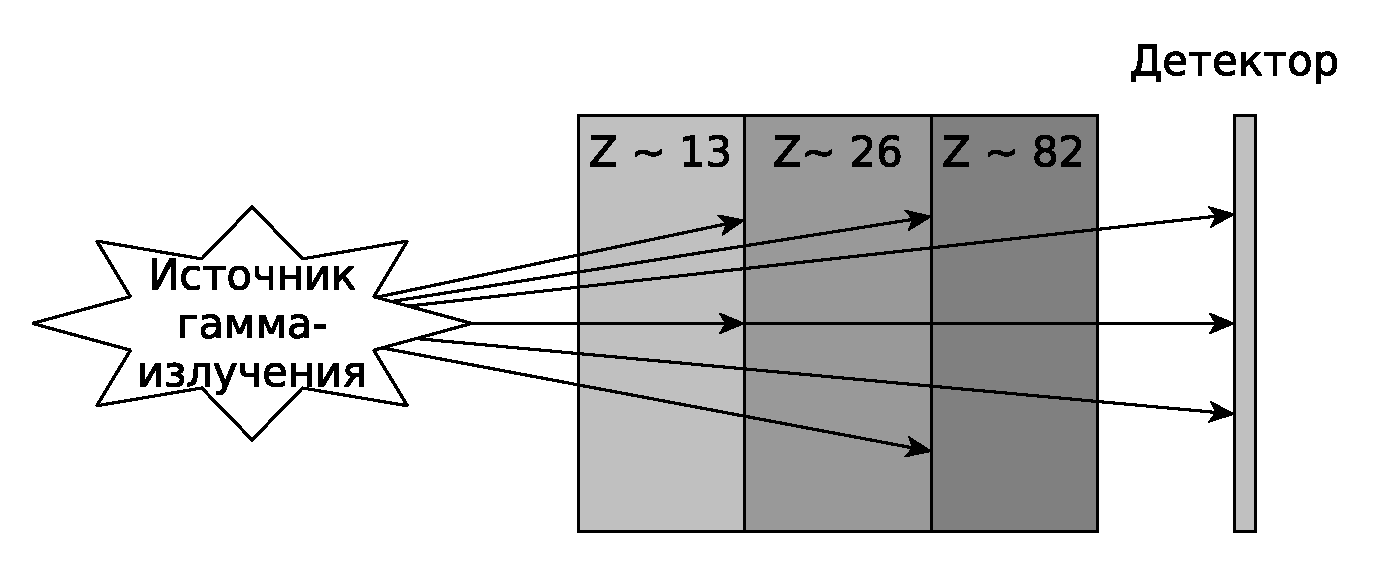
\includegraphics[width=\linewidth]{scanner/yed_schema_2.pdf}
    \caption{Восстановление толщин материалов (схема моделирования).}
    \label{schema2}
}
\end{figure}
Рисунок~\ref{rec:ex}б показывает разброс ошибки восстановления для данных наборов. Как мы можем видеть толщина тяжелых элементов определяется лучше всего: с точность порядка 5\%, а толщина элементов из группы железа хуже всего: величина ошибки достигает 30\%. Однако, мы рассматривали весьма простую модель и возникает вопрос: какая от неё польза? В данной модели мы использовали только энергетическое разрешение и по нему смогли провести восстановление послойной структуры объекта. При добавлении пространственного распределение, мы можем провести дополнительно сегментирование вдоль ещё одной оси и с учетом временной компоненты восстановить трехмерную структуру груза контейнера (3D гамма-томография). Таким образом наша простая модель показывает, что у нас есть перспектива создания действительно мощной системы для анализа содержимого контейнеров.

\begin{figure}[t]
    \begin{center}
        \begin{minipage}[h]{0.49\linewidth}
            \center{\includegraphics[width=0.99\linewidth]{scanner/reconstruction.pdf} \\ а)}
        \end{minipage}
        \hfill
        \begin{minipage}[h]{0.49\linewidth}
            \center{\includegraphics[width=0.99\linewidth]{scanner/relError.pdf}   \\ б)}
        \end{minipage}
        \caption{а) Вклад отдельных слоев в полное ослабление потока. б) Распределение ошибок восстановления для различных численных экспериментов.}
    \end{center}
    \label{rec:ex}
\end{figure}

\begin{table}
    \caption{Пример результата  работы алгоритма восстановления}
    \label{tab:rec}
    \begin{center}
        \begin{tabular}[c]{|c|c|c|}
            \hline 
            Материал & Истинная толщина, см & Восстановленная, см \\ 
            \hline 
            Al & 20 & 19.6 \\ 
            \hline 
            Fe & 40 & 41.6 \\ 
            \hline 
            Pb & 30 & 28.7 \\ 
            \hline 
        \end{tabular}
    \end{center}
\end{table}

\newpage
\subsection{Измерение энергетического разрешения детектора}
В дополнение к моделированию, было измерено энергетическое разрешение сцинтилляционного детектора гамма-излучения. В качестве сцинтиллятора использовался кристалл BGO размером 10x30x100~мм (глубина кристалла подбиралась так, чтобы обеспечить полное поглощение гамма-квантов до 10~МэВ), для регистрации излучения сцинтиллятора использовался фотодетектор ArrayC-60035-4P. В качестве источников излучения использовались $^{22}Na$ (имеет две линии 0.511~МэВ и 1.275~МэВ) и $^{137}Cs$ (имеет линию 0.662~МэВ). Фотодетектор ArrayC-60035-4P  представляет из себя матрицу из четырёх фотодиодов размером 6x6~мм, оснащенную индивидуальным предусилителем с коэффициентом усиления равным 150. В процессе работы измерялся суммарный сигнал с двух фотодиодов матрицы. Сигнал c матрицы подавался на усилитель (ORTEC~579) и затем поступал на входной канал АЦП (CAEN~DT5742) и на дискриминатор (CAEN mod. 224), логический сигнал которого служил триггером в системе. В отсутствие источника шкала АЦП была прокалибрована в абсолютных единицах --- числе фотоэлектронов. В таблице~\ref{tab:ex} представлен результат измерения разрешения детектора ---  отношения СКО фотопика к его положению ($\frac{\sigma_E}{E}$). Световыход составляет 140 фотоэлектронов на МэВ, а порог шумов --- величину порядка 100~кэВ.\\
\begin{table}
    \caption{Измерение энергетического разрешения детектора}
    \label{tab:ex}
    \begin{center} 
        \begin{tabular}[c]{|c|c|c|}
            \hline 
            Источник & Энергия, МэВ & $\frac{\sigma_E}{E}$\\
            \hline 
            $^{22}Na$&0.511 & 19.0 \%  \\ 
            \hline 
            $^{137}Cs$&0.662 & 14.7\%\\ 
            \hline 
            $^{22}Na$& 1.275 & 13\% \\
            \hline 
        \end{tabular} 
    \end{center}
\end{table}


\subsection{Обобщение результатов и обсуждение дальнейших перспектив разработки}
Результаты:   
\begin{enumerate}
    \item Энергетические спектры материалов с различным эффективным зарядовым числом различаются в областях энергий до 3 и после 4~МэВ. Оценена зависимость зарядового числа от доли гамма-квантов с энергией выше 3~МэВ. Данный метод позволяет идентифицировать в контейнере отдельные группы элементов по зарядовому числу (легкие, средние, тяжелые) в одной экспозиции при одной фиксированной энергии электронов, оптимально вблизи 8~МэВ. При этом требуется разрешение не хуже 15\% и эффективность регистрации около 90\%. 
    \item Энергетическое разрешение порядка 10\% позволяет определить толщину отдельного слоя в многослойной структуре с точностью 25\%.
    \item Измерено энергетическое разрешение детектора на основе BGO, в целом полученные результаты говорят о высоких эксплуатационных характеристиках и качестве материала. Представляется возможным достижение характеристик заявленных производителем ($FWHM \sim 9\%$ для $^{137}Cs$).
\end{enumerate}

Развитие данной тематике является перспективным направлением деятельности, но требует финансовой поддержки, при наличии которой становиться возможным разработка программы для проверки содержимого транспортного контейнера по заявленному манифесту, и создание программы для гамма-томографии содержимого контейнеров.
